\section{Portability and extendibility}

Software design patterns are standardized solutions to common problems encountered in software design. 
They serve as reusable templates that can be adapted to address recurring challenges in code structure and implementation. 
In OS design, patterns play a significant role. Two of the most commonly employed patterns in OS design are the Facade and Bridge patterns, which help simplify and manage system complexity.

\subsection{Facade}
The Facade pattern provides a simplified interface to a complex subsystem, which may have many intricate components. 
While the facade typically offers limited functionality compared to interacting with the subsystem directly, it focuses on exposing only the features that are essential and relevant to the client.

For example, a system call to write to a file abstracts the complexity of interacting with the appropriate hardware device at the low level, making the interaction easier for the developer.
\begin{figure}[H]
    \centering
    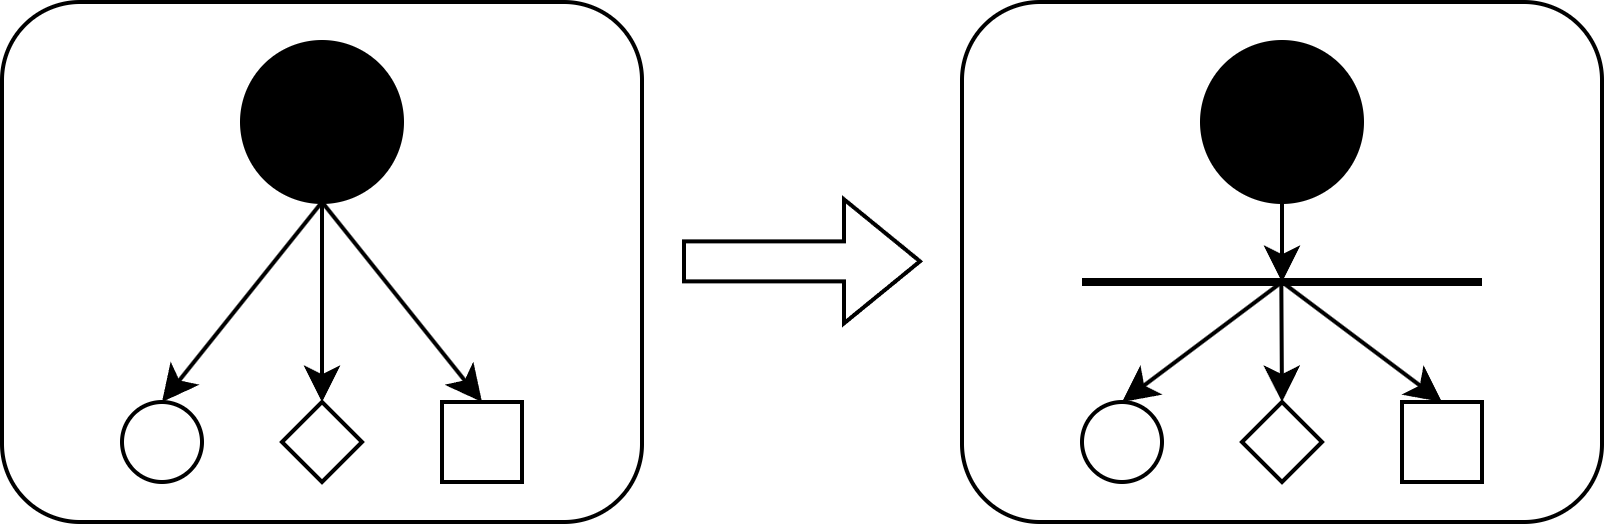
\includegraphics[width=0.75\linewidth]{images/facade.png}
    \caption{Facade pattern}
\end{figure}
The Facade pattern is useful when a simpler, higher-level interface to an underlying system is desired. 
It often exposes only high-level APIs and hides the lower-level complexities. This pattern is implemented using exceptions and is commonly seen in system calls.

\paragraph*{System calls}
A system call (syscall) is a mechanism that allows an application to request a privileged service from the operating system's kernel. 
Since applications run in an unprivileged mode, they rely on system calls to perform tasks that require higher privileges.

When a system call is invoked, a special instruction triggers an exception that transfers control to the kernel, allowing it to process and validate the request. 
This is similar to a library call but occurs in the more privileged kernel code.

System calls are identified by numbers listed in a syscall table. 
The system call number, along with its function parameters, is placed in designated CPU registers before the call is executed.

On Linux systems, you can observe the system calls made by a process using the \texttt{strace} tool in real time.
\begin{figure}[H]
    \centering
    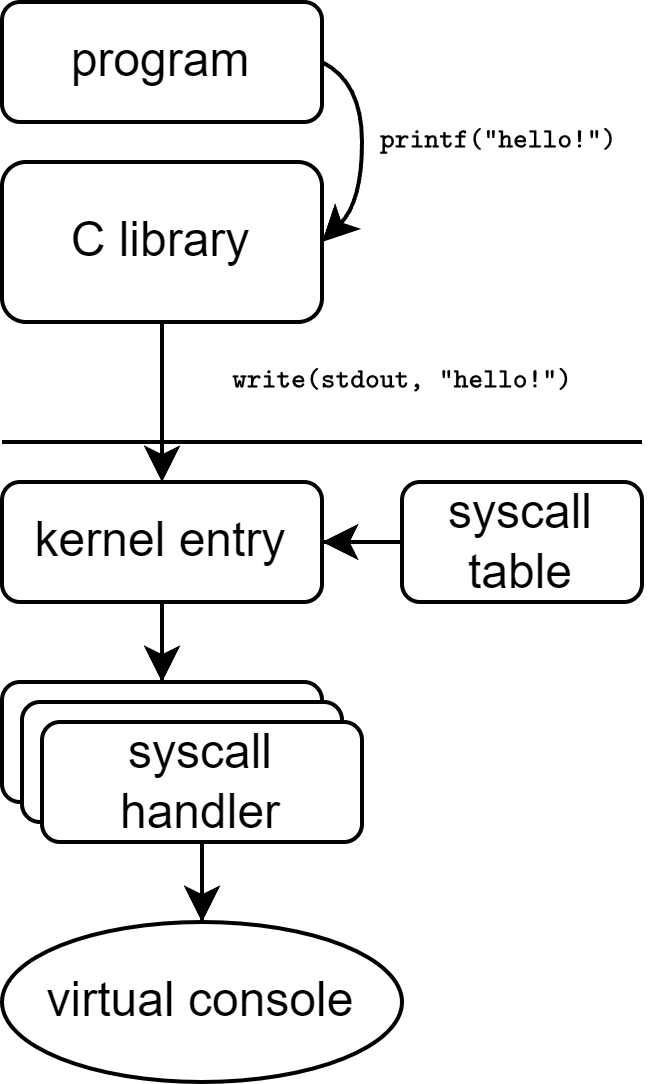
\includegraphics[width=0.3\linewidth]{images/syscall.png}
    \caption{System call}
\end{figure}

\subsection{Bridge}
The Bridge pattern is designed to decouple an abstraction from its implementation, allowing both to be defined and extended independently. 
This separation enables flexibility, as the implementation can be selected or changed at runtime, rather than being fixed at compile time.

For example, in operating systems like Unix, the way the file system hierarchy is structured and exposed should remain independent of the actual file system being used (e.g., ext4, NTFS, FAT32). 
This allows different file systems to be mounted without modifying the core abstraction of the file system interface.
\begin{figure}[H]
    \centering
    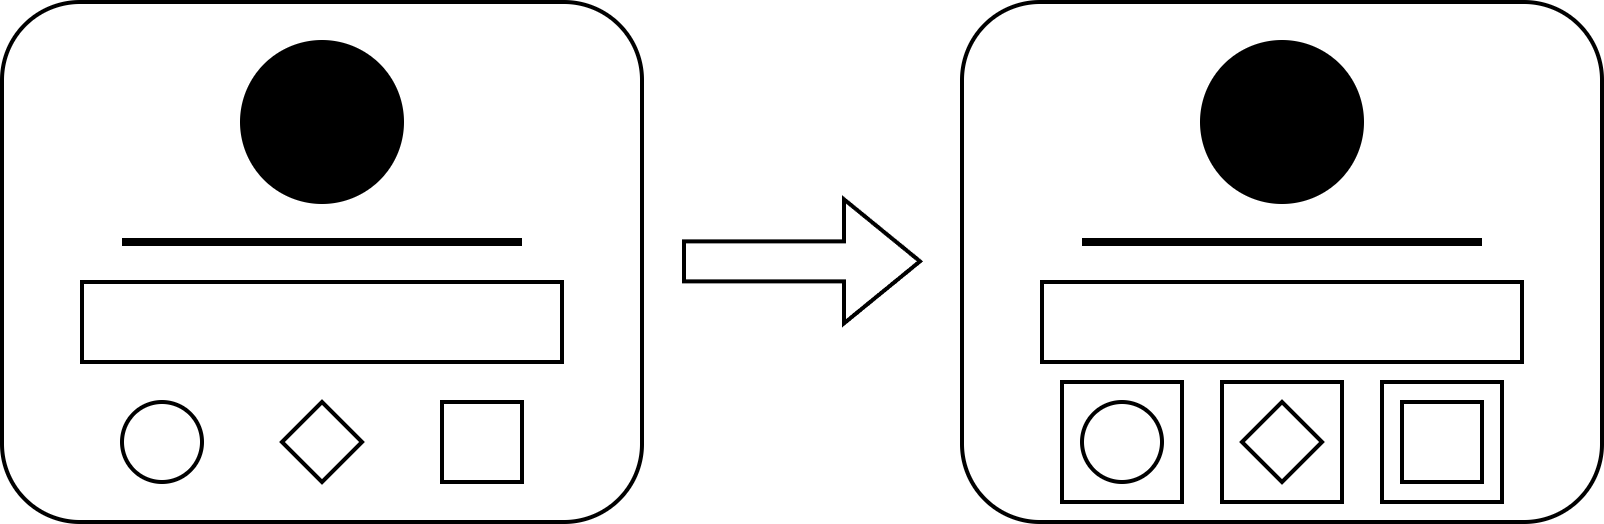
\includegraphics[width=0.75\linewidth]{images/bridge.png}
    \caption{Bridge pattern}
\end{figure}
The Bridge pattern is particularly useful for organizing monolithic code that contains multiple variations of functionality. 
It divides the abstraction and its variants, improving modularity and maintainability. 
This pattern is commonly implemented using virtual classes and interfaces, and it is often used in file systems and peripheral drivers.

\paragraph*{File system}
A file system is a set of mechanisms and policies used to manage access to persistent storage. 
It operates across multiple storage devices (such as hard drives, SSDs, RAM, and network storage) and supports various formats (e.g., FAT32, NTFS, ext2, ext3, ext4). 
The file system allows multiple processes to access storage concurrently while ensuring data integrity and security.
The primary goals of a file system include providing:
\begin{itemize}
    \item A common abstraction for storage devices.
    \item Efficient space management.
    \item Protection and security for stored data.
\end{itemize}

\begin{figure}[H]
    \centering
    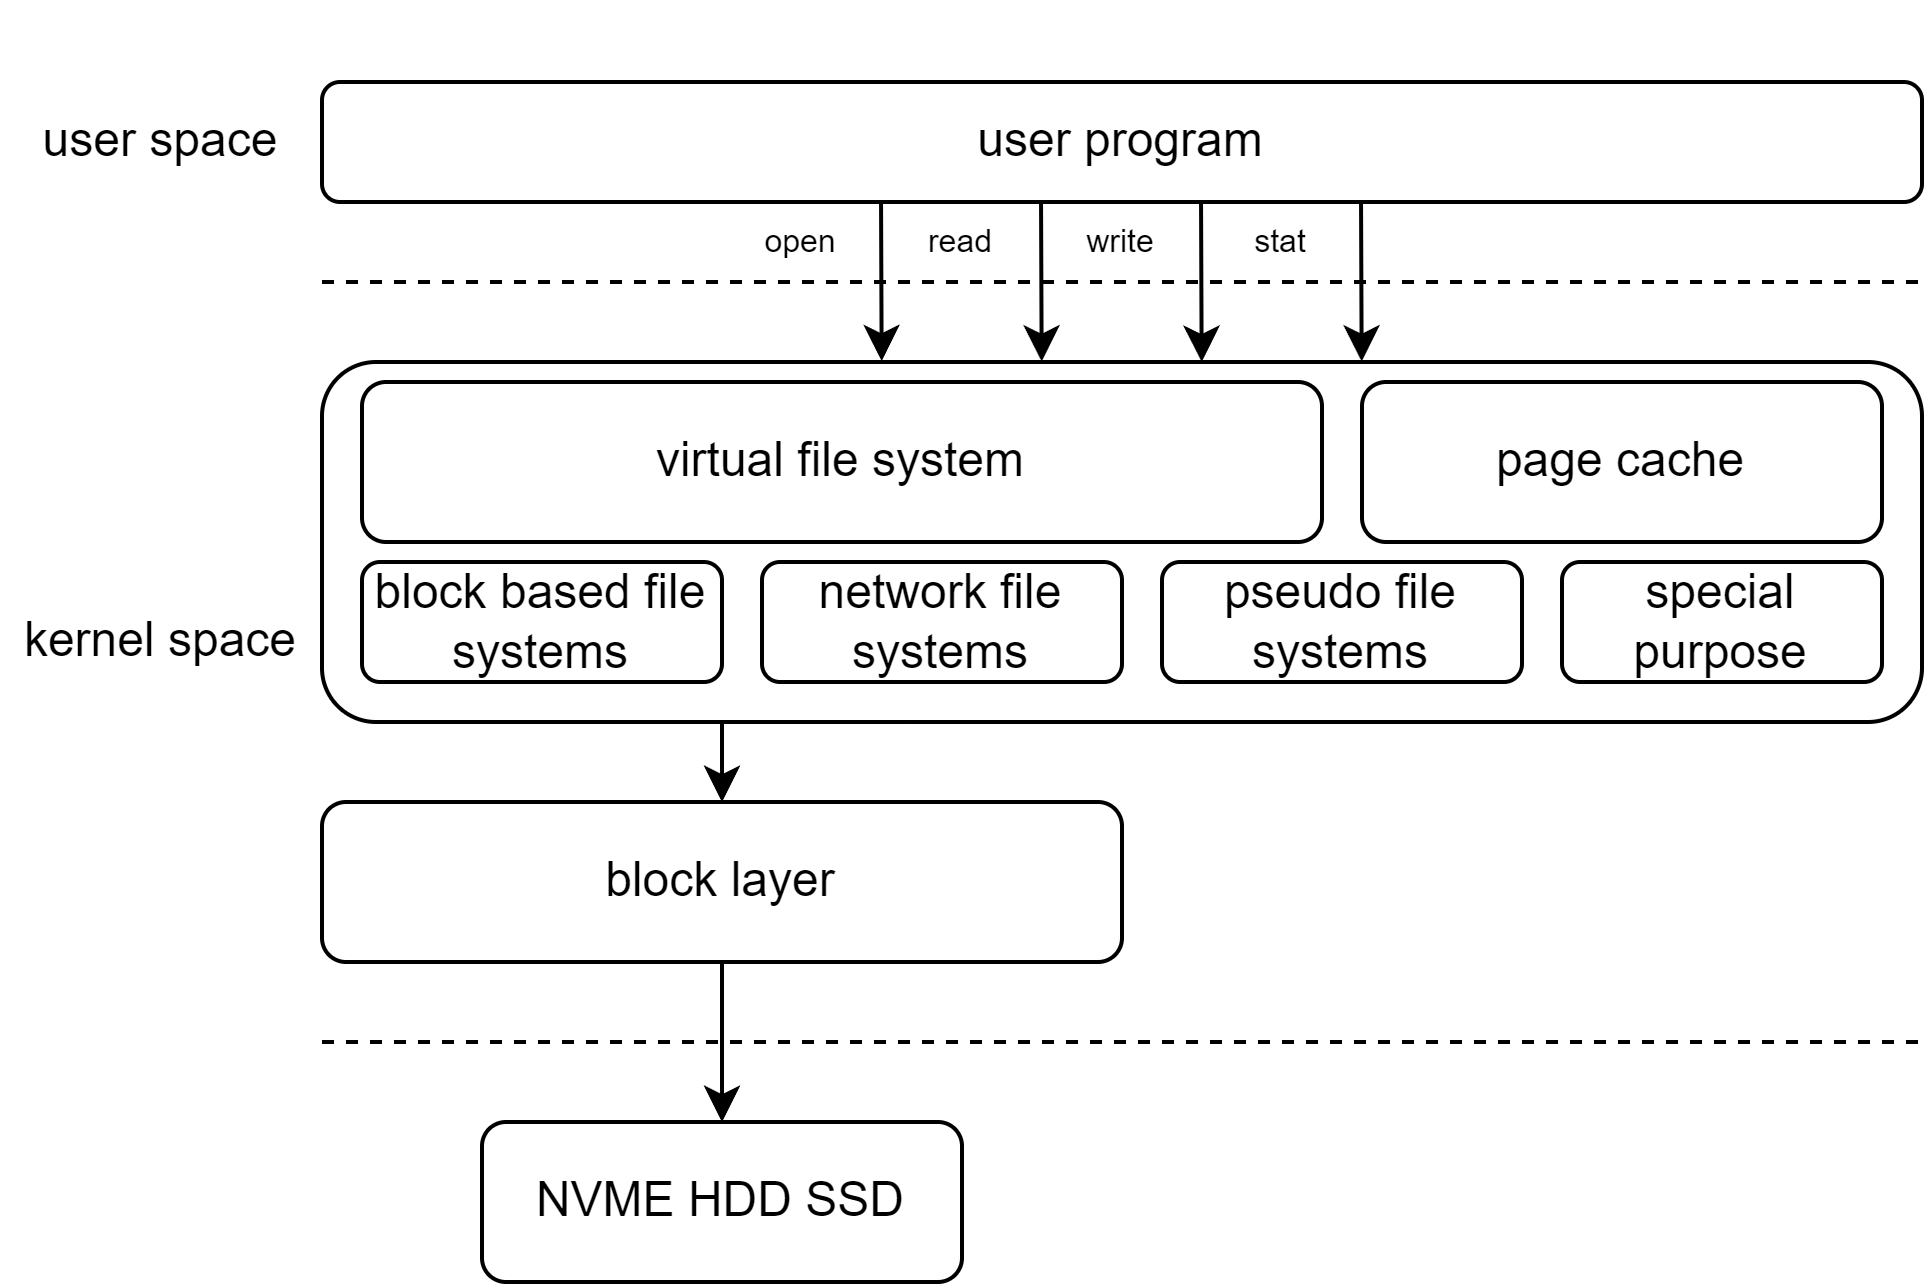
\includegraphics[width=0.75\linewidth]{images/fs.png}
    \caption{File system}
\end{figure}

\subsection{Other patterns}
Operating systems also utilize various behavioral design patterns to manage complex interactions and processes. 
Some of the key patterns used are:
\begin{itemize}
    \item \textit{Chain of Responsibility}: the Chain of Responsibility pattern allows a request to be passed along a chain of handlers. 
        Each handler in the chain decides whether to process the request or pass it on to the next handler. 
        This approach helps distribute the responsibilities and makes the system more flexible.
        For instance, in file systems, when serving data for a file, the request might first check if the data is available in a cache. 
        If not, it passes the request to the disk for retrieval.
    \item \textit{Command}: the Command pattern encapsulates a request as a stand-alone object that contains all necessary information about the request. 
        This allows requests to be passed as method arguments, queued for later execution, or even undone if needed. 
        It is particularly useful for decoupling the sender of the request from the receiver.
        For instance, block I/O requests in an operating system can be queued or delayed, allowing for more control over their execution. 
        Additionally, undoable operations can be implemented using this pattern, enabling rollback in case of failure.
\end{itemize}